% TEX compiler = latexmk
% copyright arturo salinas-aguayo 2024
\documentclass[12pt]{article}

\usepackage{graphicx}
\usepackage{amsmath}
\usepackage{array}
\usepackage{amsfonts}
\usepackage{fancyhdr}
\usepackage{geometry}
\usepackage{circuitikz}
\usepackage{subfigure}
\usepackage{caption}
\usepackage{karnaugh-map}
\usepackage{bm}
\usepackage[table]{xcolor}
\usepackage{float}
\usepackage{subcaption}

\geometry{letterpaper, margin=1in}
\graphicspath{ {../images/} }

% Header and Footer
\pagestyle{fancy}
\fancyhf{}
\fancyhead[L]{CSE 2301 - Lab 12: VHDL}
\fancyhead[R]{\thepage}
\setlength{\headheight}{15pt}

\author{Arturo Salinas-Aguayo}
\title{Lab 12: VHDL}
% theorem set
\newtheorem{example}{Example}
% Example block environment
\newenvironment{examp}
{
	\vspace{.5cm}
	\hrule
\begin{example}\upshape}
	{\hrule
		\vspace{0.5cm}
\end{example}}

\begin{document}
\newcommand{\closure}[2][3]{%
	{}\mkern#1mu\overline{\mkern-#1mu#2}}
\newcommand\ncoverline[1]{\mkern1mu\overline{\mkern-1mu#1\mkern-1mu}\mkern1mu}
% Title Page
\begin{titlepage}
	\centering
	\vspace*{3cm}
	\huge\textbf{Lab 12: VHDL}\\
	\vspace{5cm}
	\Large\textbf{Arturo Salinas-Aguayo}\\
	\normalsize
	CSE 2301: Principles and Practice of Digital Logic Design\\
	Dr. Mohammad Khan, Section 003L-1248\\
	Electrical and Computer Engineering Department
	\vfill
	
\includegraphics[scale=0.1]{uconnlogo}\\
	College of Engineering, University of Connecticut\\
	\scriptsize{Coded in \LaTeX}
	\vspace*{1cm}
\end{titlepage}
\section*{Discussion}
This lab introduced the concept of a Hardware Description Language in order to
synthesize logic. VHDL stands for \textit{Very High Speed Hardware Description
	Language} and was standardized by the IEEE for digital circuit production.
\begin{examp}
	\vspace{.5cm}
	\textbf{The Hamming Parity Error Check in VHDL}\\
	\begin{verbatim}
library IEEE;
use IEEE.std_logic_1164.all;


entity ParityGen is 

 port(
		D	: in	std_logic_vector(3 downto 0);
		Q	: out	std_logic_vector(6 downto 0)
	);

end ParityGen;

architecture arch1 of ParityGen is
signal P1 : std_logic;
signal P2 : std_logic;
signal P3 : std_logic;
begin
	Q(6) <= P1;
	Q(5) <= P2;
	Q(4) <= D(3);
	Q(3) <= P3;
	Q(2) <= D(2);
	Q(1) <= D(1);
	Q(0) <= D(0);
	
	P1 <= Q(0) XOR Q(2) XOR Q(4); 
	P2 <= Q(4) XOR Q(1) XOR Q(0); 
	P3 <= Q(2) XOR Q(1) XOR Q(0); 

end arch1;
		\end{verbatim}
\end{examp}
\begin{examp}
	\vspace{.5cm}
	\textbf{The ALU Reprise}\\
	\begin{verbatim}
library IEEE;
use IEEE.std_logic_1164.all;
use IEEE.numeric_std.all;

entity ALU2ElectricBoog is 

 port(
		B	: in	std_logic_vector(1 downto 0);
		A	: in	std_logic_vector(1 downto 0);
		Q	: out	std_logic_vector(3 downto 0);
		Op	: in	std_logic_vector(1 downto 0)
	);

end ALU2ElectricBoog;

architecture arch1 of ALU2ElectricBoog is
begin
	process (A, B, Op)
    begin
    	if Op = "00" then
    		Q <= "00" & A and "00" & B;
    	elsif Op = "01" then
                Q <= "00" & A or "00" & B;
    	elsif Op = "10" then
    		Q <= unsigned("00" & A) + unsigned("00" & B);
    	elsif Op = "11" then
                Q <= unsigned(A) * unsigned(B);
    	end if;
    end process;
end arch1;

	\end{verbatim}
\end{examp}
\begin{examp}
\vspace{.5mm}
\subsection*{The Use of \texttt{unsigned()} Cast}

The \texttt{unsigned()} function in VHDL is used to cast a binary vector to an \texttt{UNSIGNED} type, treating the vector as a positive integer. This explicit casting allows VHDL to interpret binary data without ambiguity, particularly during arithmetic operations, ensuring that the result is processed as an unsigned value. In VHDL, operations between \texttt{SIGNED} and \texttt{UNSIGNED} types require conversions to maintain compatibility, as VHDL does not implicitly mix these types.

In the context of your ALU code:
\begin{itemize}
	\item \textbf{\texttt{unsigned()}} ensures that \texttt{A} and \texttt{B} are interpreted as positive integers, allowing for correct behavior in operations like addition (\texttt{+}) without treating them as potentially negative numbers.
\end{itemize}

\section*{Effect of Using \texttt{signed()} Instead of \texttt{unsigned()}}

If you were to replace \texttt{unsigned()} with \texttt{signed()} in the ALU, the output could change significantly, particularly in cases where \texttt{A} or \texttt{B} have high bits set to \texttt{1} (interpreted as negative in 2’s complement). For example:
\begin{itemize}
	\item With \textbf{\texttt{unsigned}}, a binary vector such as \texttt{"1100"} would be interpreted as \(12\).
	\item With \textbf{\texttt{signed}}, the same vector \texttt{"1100"} would be interpreted as \(-4\) in 2's complement form.
\end{itemize}

This change would result in different outputs for operations that involve addition or multiplication, where the result might switch from a positive to a negative value, depending on the high bits of the input.

\section*{Circuit Element Emulated by \texttt{if} and \texttt{elsif} Statements}

In the ALU, the \texttt{if} and \texttt{elsif} statements emulate the behavior of a \textbf{multiplexer (MUX)}. The \texttt{Op} input acts as a selector that determines which operation (AND, OR, ADD, or MULTIPLY) the ALU will perform based on its value. Each condition (e.g., \texttt{Op = "00"}, \texttt{Op = "01"}, etc.) corresponds to a specific operation, similar to how a multiplexer selects an output based on control signals.
\begin{center}
\begin{karnaugh-map}(label=corner)[4][4][2][$B$][$A$][$C_0$][$C_1$][$C_2$]
\minterms{0,1,2,3,5,6,7,8,9,10,13,14,16,19,23,24}
\implicant{1}{9}
\implicant{2}{10}
\implicant{3}{7}[0,1]
\implicantedge{0}{0}{8}{8}[0,1]
\autoterms[0]
\end{karnaugh-map}
\end{center}
\[
	F = \closure{C_0}\closure{A}\closure{B} + \closure{C_1}AB +
	\closure{C_2}\closure{A}B + \closure{C_2}A\closure{B}
\]
With the PLA implementation, each minterm for each output bit is placed and
routed by the software and abstracted away from the wires. For the \(C_2 = 0\)
block, notice how there are potential hazards at bay. These are kept seperate in
order to best maximize the effect of the 3-Dimensional 5 Variable Karnaugh Map.
In this case, the blue and yellow squares ``wrap around" the corresponding
\(C_2\) block.
\begin{figure}[H]
	\center{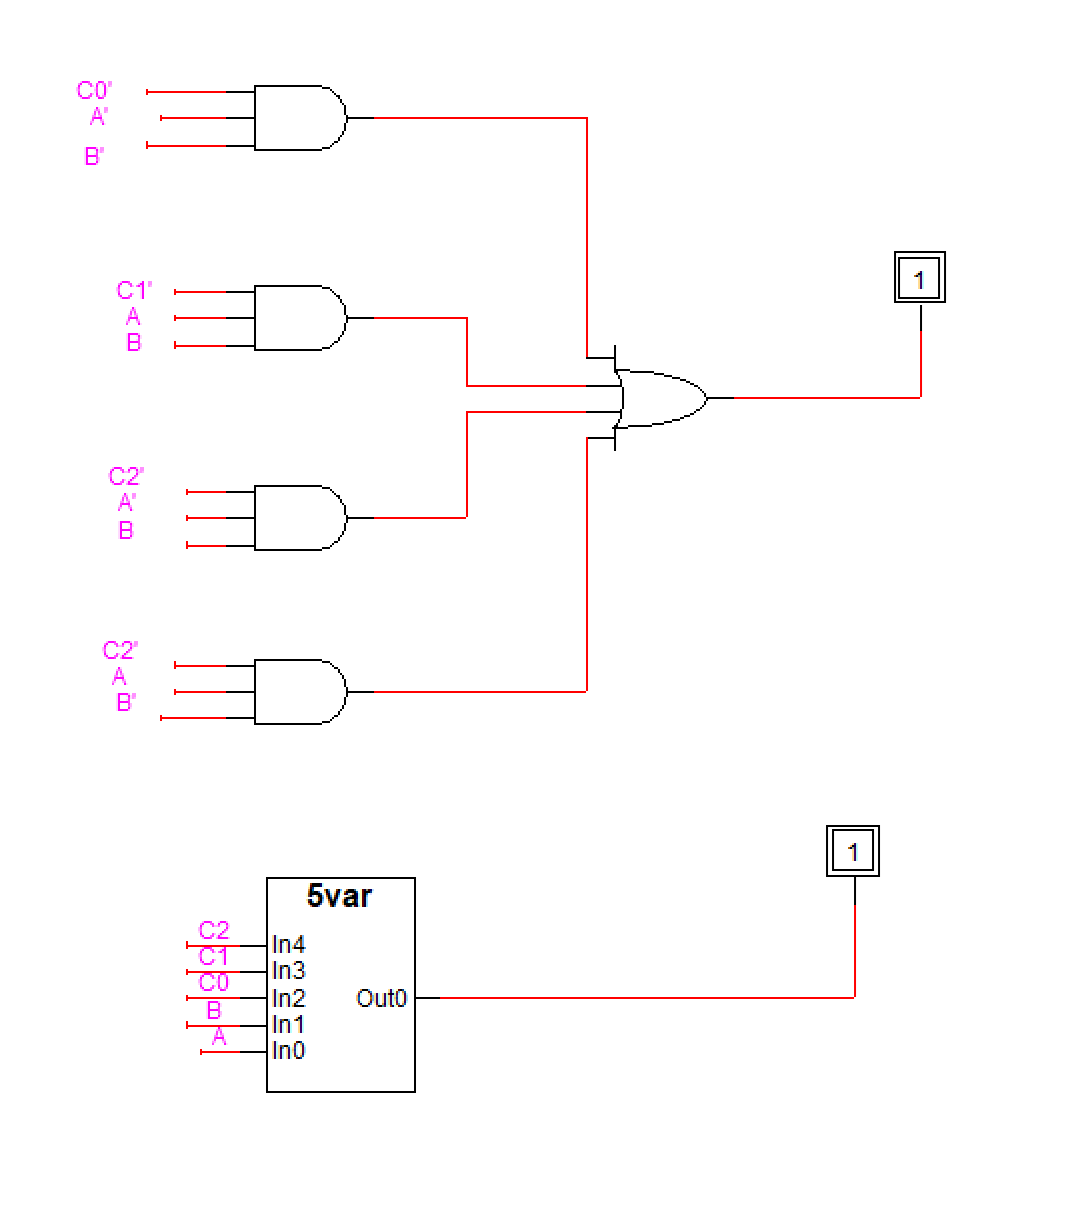
\includegraphics[scale=.60]{examp113}}
	\caption{Traditional Gate Implementation and Black Box
		Implementation}
\end{figure}
The PLA form greatly reduces the complexity of visual schematic design by
abstracting away the gate logic by programming it directly.
\end{examp}

\begin{examp}
	\vspace{.5mm}
	\textbf{A Continuation of the Triangle Parity}

	In this lab, we examined a 15-bit data stream configured with EVEN parity using a triangular code. The output identifies error positions by mapping the detected location to a four-bit decimal representation. An error is flagged whenever a mismatch in parity is detected across specific bit groupings, similar to Hamming code principles. Recall that in a Hamming code, the minimum number of parity bits \( p \) needed for \( m \) data bits satisfies \( 2^p \geq m + p + 1 \). This ensures unique identification of single-bit errors. The triangular parity code, however, uses overlapping parity checks to pinpoint errors more precisely by leveraging redundancy within intersecting bit groups.
	\begin{table}[H]
		\centering
		\newcommand{\currstatecolor}{gray!30}
		\begin{tabular}{|c|c|c|c|c
			|>{\columncolor{\currstatecolor}}c
			|>{\columncolor{\currstatecolor}}c
			|>{\columncolor{\currstatecolor}}c
			|>{\columncolor{\currstatecolor}}c
			|l|}
			\hline
			\textbf{A} & \textbf{B} & \textbf{C} & \textbf{D} & \textbf{E} & \textbf{F} & \textbf{G} & \textbf{H} & \textbf{I} & \textbf{Error Position} \\ \hline
			0          & 0          & 0          & 0          & 0          & 0          & 0          & 0          & 0          & None (No Error)         \\ \hline
			1          & 0          & 0          & 0          & 0          & 0          & 1          & 0          & 1          & Parity Bit 5            \\ \hline
			1          & 1          & 0          & 0          & 0          & 0          & 1          & 0          & 0          & Data Bit 4              \\ \hline
			1          & 0          & 1          & 0          & 0          & 0          & 0          & 1          & 1          & Data Bit 3              \\ \hline
			1          & 0          & 0          & 1          & 0          & 0          & 0          & 1          & 0          & Data Bit 2              \\ \hline
			1          & 0          & 0          & 0          & 1          & 0          & 0          & 0          & 1          & Data Bit 1              \\ \hline
			0          & 1          & 0          & 0          & 0          & 1          & 0          & 0          & 1          & Parity Bit 9            \\ \hline
			0          & 1          & 1          & 0          & 0          & 1          & 0          & 0          & 0          & Data Bit 8              \\ \hline
			0          & 1          & 0          & 1          & 0          & 0          & 1          & 1          & 1          & Data Bit 7              \\ \hline
			0          & 1          & 0          & 0          & 1          & 0          & 1          & 1          & 0          & Data Bit 6              \\ \hline

			0          & 0          & 1          & 0          & 0          & 1          & 1          & 0          & 0          & Parity Bit 12           \\ \hline
			0          & 0          & 1          & 1          & 0          & 1          & 0          & 1          & 1          & Data Bit 11             \\ \hline
			0          & 0          & 1          & 0          & 1          & 1          & 0          & 1          & 0          & Data Bit 10             \\ \hline
			0          & 0          & 0          & 1          & 0          & 1          & 1          & 1          & 0          & Parity Bit 14           \\ \hline
			0          & 0          & 0          & 1          & 1          & 1          & 1          & 0          & 1          & Data Bit 13             \\ \hline
			0          & 0          & 0          & 0          & 1          & 1          & 1          & 1          & 1          & Parity Bit 15           \\ \hline
		\end{tabular}
		\caption{Truth Table for Error Detection (5 Inputs, 4 Outputs)}
	\end{table}
\end{examp}
\begin{examp}
	\vspace{.5mm}
	\textbf{The Overflow of a 3 bit by 3 bit full Adder}\\
	\begin{figure}[H]
		\center{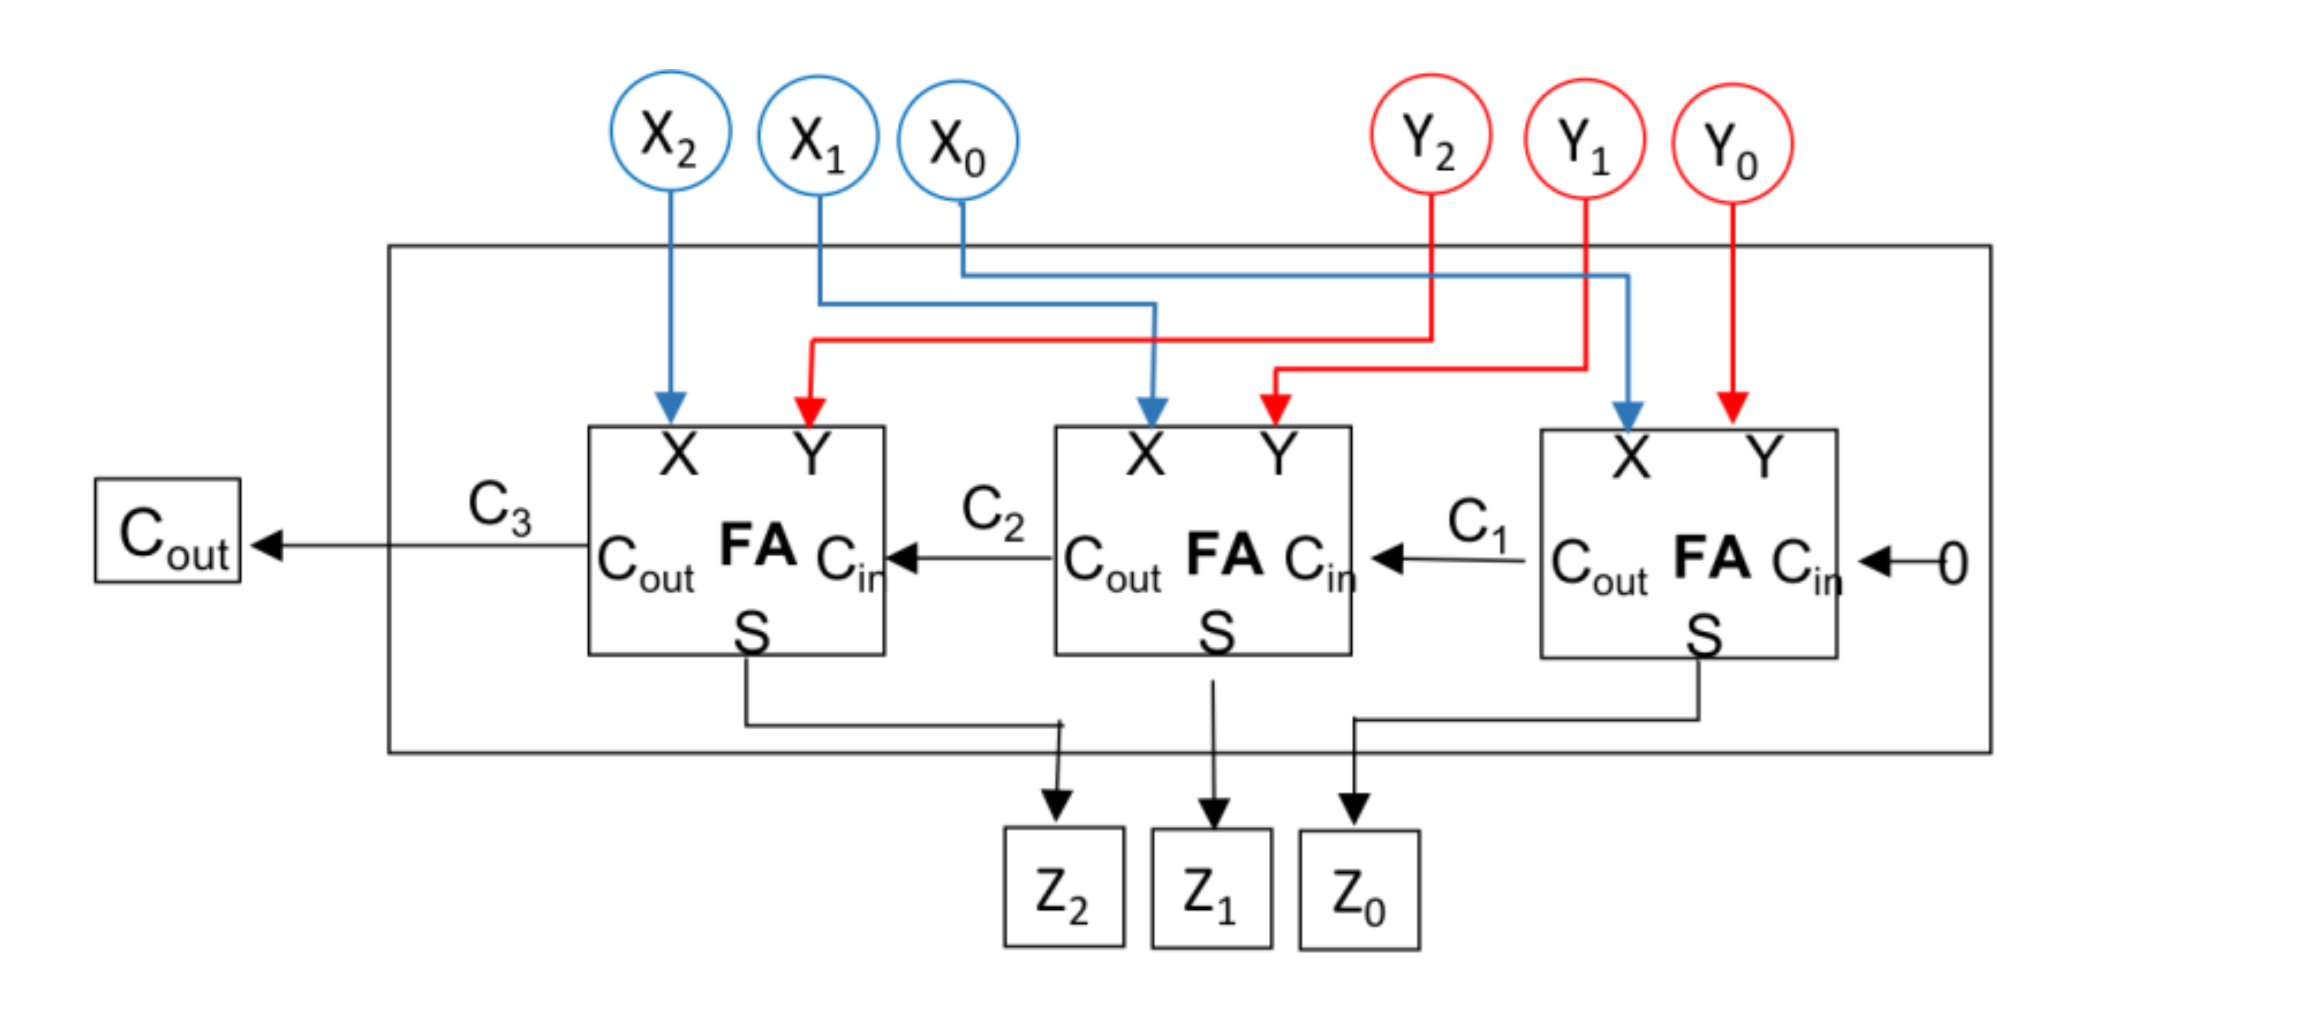
\includegraphics[scale=.60]{examp111}}
		\caption{The 3x3 bit Full Adder Circuit}
	\end{figure}

	The output \textbf{OVERFLOW} bit, which can be used as a signal for the logic
	to indicate a potentially erroneous operation, can be determined quickly by comparing the MSB of Y and
	X. The equation can simply be put as:
	\[
		\mathbf{OVERFLOW} = \closure{X_2}\closure{Y_2}Z_2 + X_{2}Y_{2}\closure{Z_{2}}
	\]

\end{examp}
\begin{examp}
	\vspace{.5mm}
	\textbf{Programmable Array Logic}\\
	For this, the task is to draw a PLA for the equation:
	\[
		F = \closure{C}A + BC
	\]
	\begin{figure}[H]
		\center{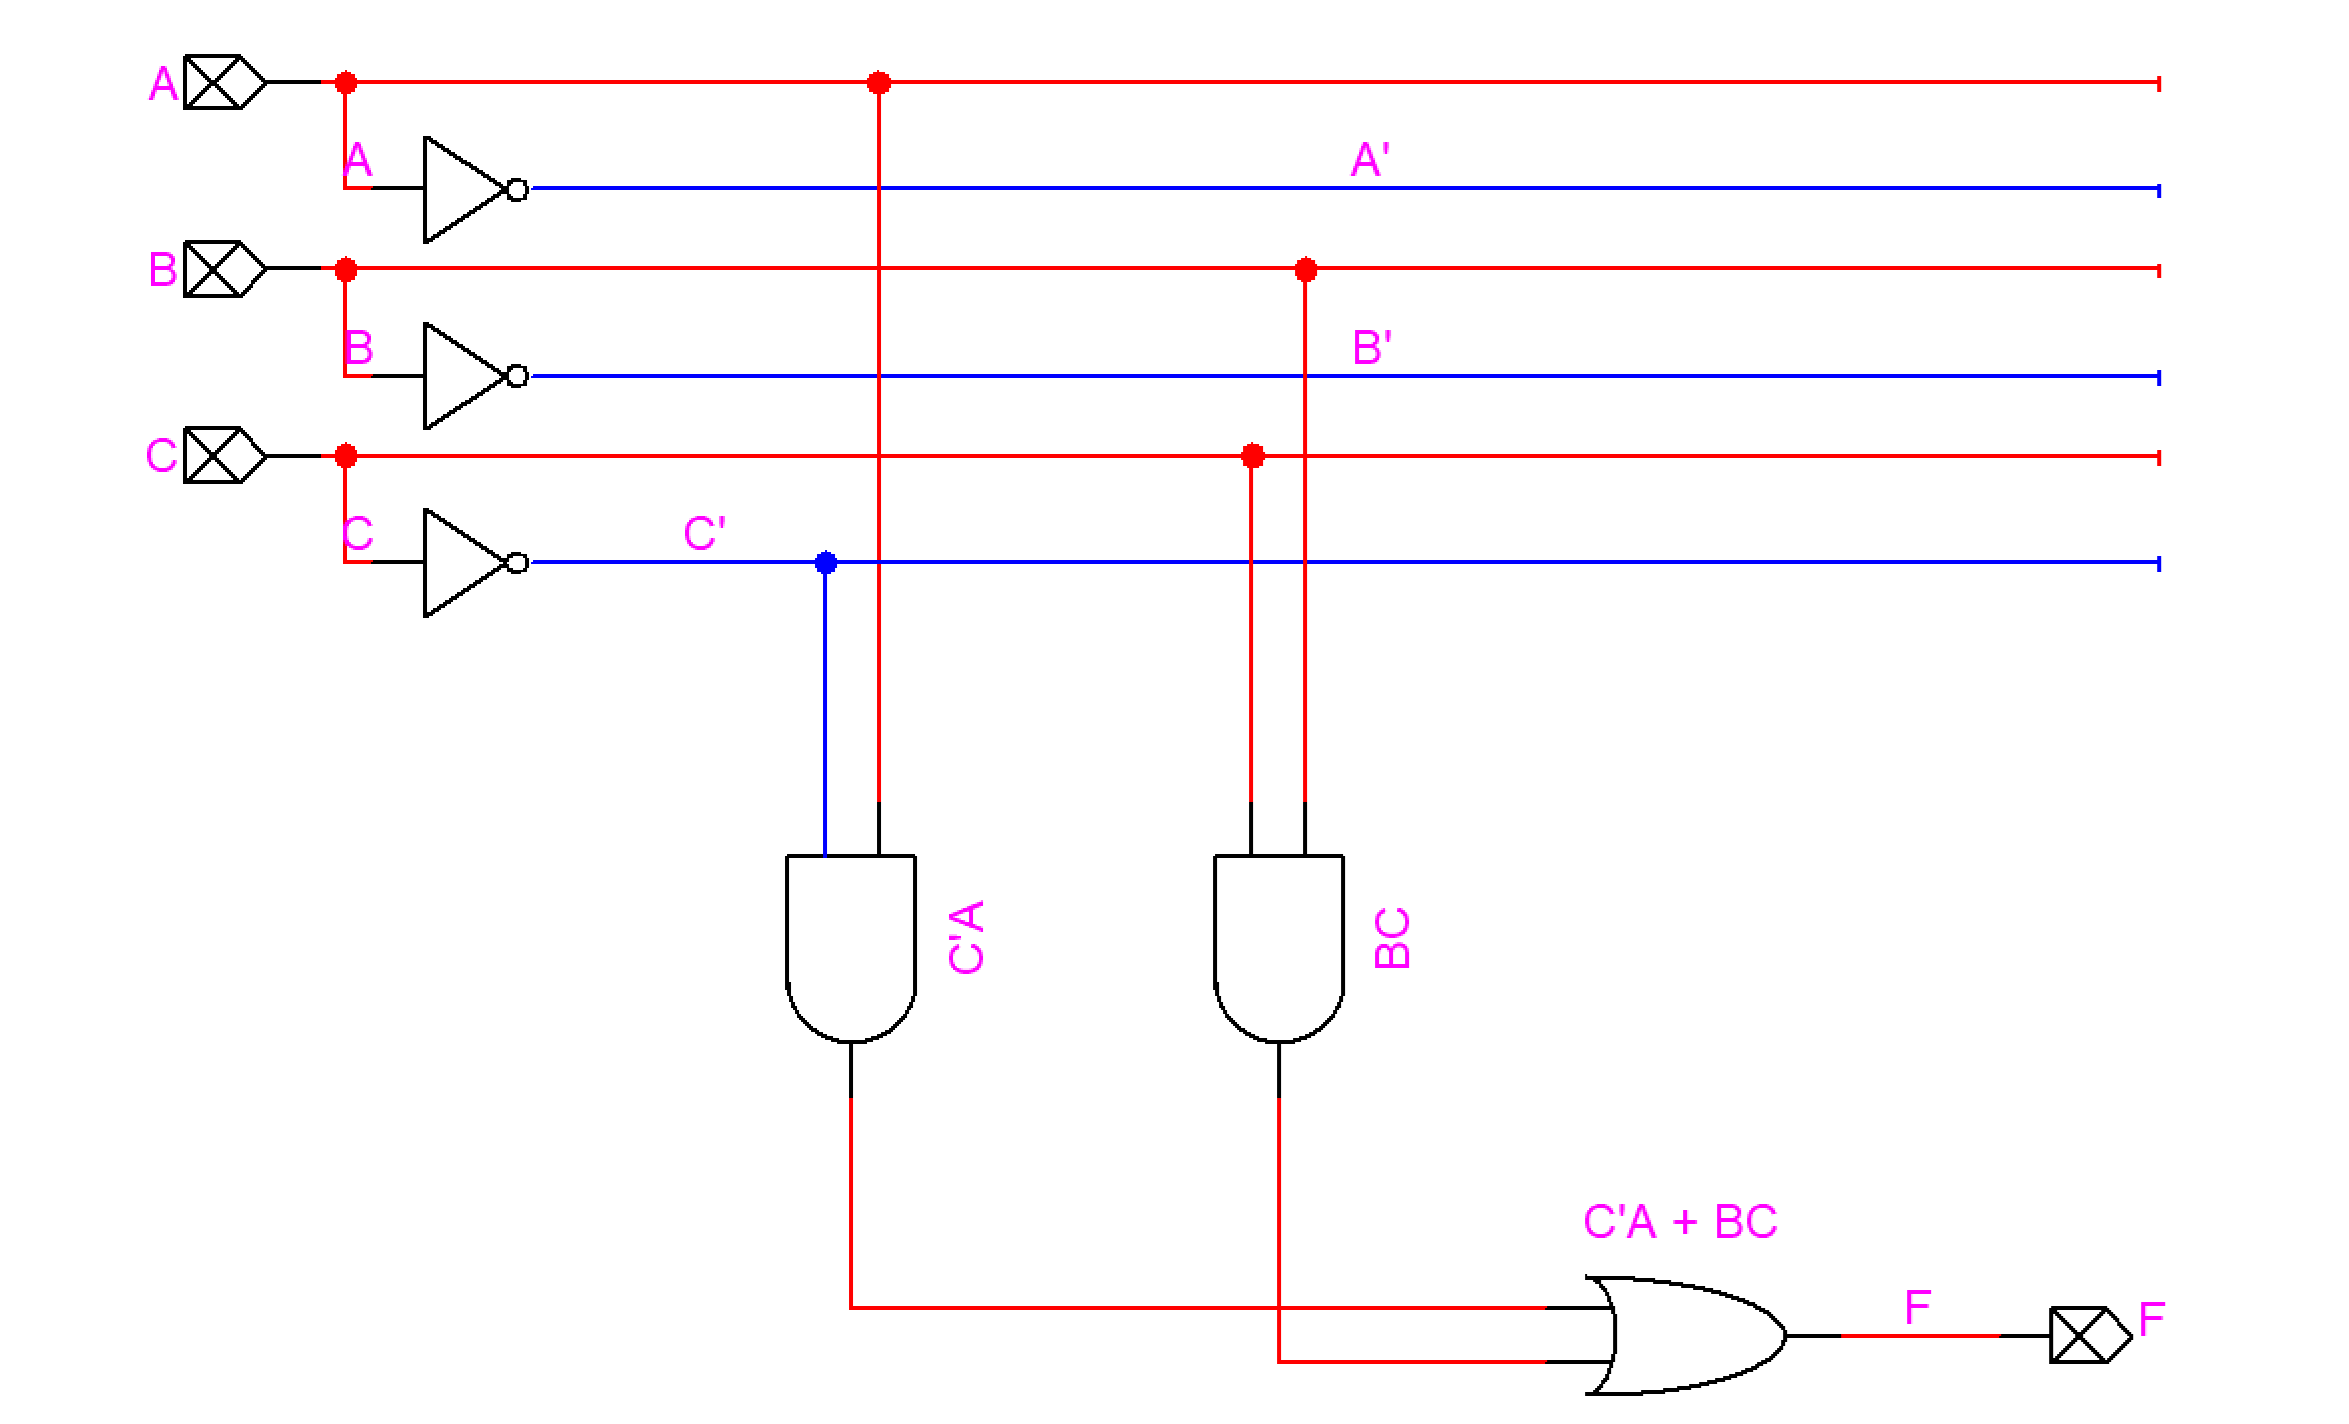
\includegraphics[scale=.50]{examp112}}
		\caption{$F = \closure{C}A + BC$}
	\end{figure}
	This is done similarly to creating combinational logic at the begining of the
	course. Every wire being drawn out and extended to the combination of AND and
	OR gates is the characteristic of the PLA.
	\vspace{5mm}
\end{examp}
\end{document}
% vim: set tw=80 ts=2 sts=2 sw=2 noai noet:
